\chapter{Arhitektura i dizajn sustava}
		
		%\textbf{\textit{dio 1. revizije}}\\

		%\textit{ Potrebno je opisati stil arhitekture te identificirati: podsustave, preslikavanje na radnu platformu, spremišta podataka, mrežne protokole, globalni upravljački tok i sklopovsko-programske zahtjeve. Po točkama razraditi i popratiti odgovarajućim skicama:}
	%\begin{itemize}
		%\item 	\textit{izbor arhitekture temeljem principa oblikovanja pokazanih na predavanjima (objasniti zašto ste baš odabrali takvu arhitekturu)}
		%\item 	\textit{organizaciju sustava s najviše razine apstrakcije (npr. klijent-poslužitelj, baza podataka, datotečni sustav, grafičko sučelje)}
		%\item 	\textit{organizaciju aplikacije (npr. slojevi frontend i backend, MVC arhitektura) }		
	%\end{itemize}
				
		Arhitektura naše aplikacije zajedno s vanjskim resursima (bazom) na najvišoj razni apstrakcije odgovara troslojnoj klijent-poslužitelj arhitekturi sa sljedećim slojevima:
		\begin{itemize}
			\item Prezentacijski sloj (Frontend)
			\item Sloj poslovne logike (Backend)
			\item Podatkovni sloj (Baza podataka)
		\end{itemize}

		\begin{figure}[H]
			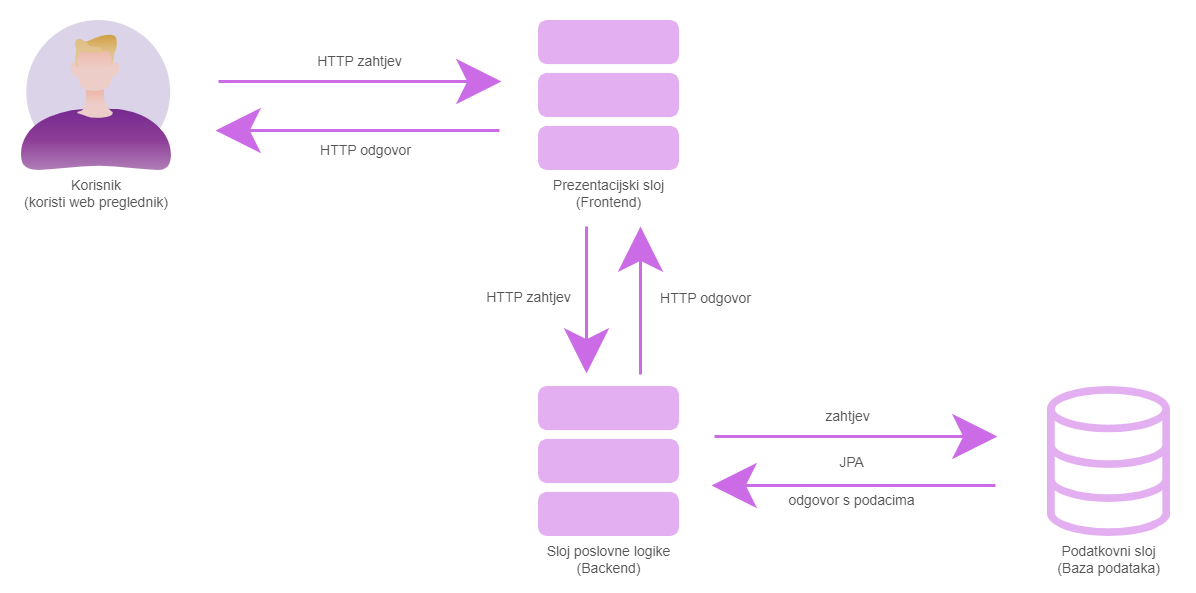
\includegraphics[width=\textwidth,height=0.4\textheight]{slike/Arhitektura.png}
			\centering
			\caption{Arhitektura sustava}
			\label{fig:Arhitektura}
		\end{figure}

		\eject

		Općenito govoreći, prezentacijski sloj tj. frontend zadužen je za prikaz stranice korisniku i omogućavanje rada s istom. S druge strane, sloj poslovne logike tj. backend zadužena je za razne izračune i interakciju s bazom. U ovom pogledu, sloj poslovne logike služi kao spona između prezentacijskog sloja i podatkovnog sloja koja pritom obavlja sve akcije neprikladne za izvođenje na klijentovom računalu.\\[2pt]

		Kada korisnik u web preglednik unese URL naše stranice, web preglednik pristupa našoj aplikaciji slanjem HTTP GET zahtjeva prezentacijskom sloju. Prezentacijski sloj u odgovoru šalje sve potrebne podatke za prikaz korisničkog sučelja - naše stranice.
		Kada korisniku treba poslužiti neki sadržaj koji nije pohranjen na prezentacijskom sloju (npr. aktivne donacije, podatci o korisniku i oglasima), prezentacijski sloj sloju poslovne logike šalje HTTP zahtjev - npr. GET zahtjev s ciljem dohvata podataka o djeci korisnika.
		Komunikacija između prezentacijskog sloja i sloja poslovne logike odvija se po REST načelima.\\[2pt]

		Sloj poslovne logike potreban je za kompliciranije izračune, dohvat i izmjenu podataka te odgovaranje na zahtjeve pristigle od strane prezentacijskog sloja.
		Podatkovni sloj tj. baza podataka služi za pohranu svih potrebnih podataka (npr. podataka o registriranim korisnicima, oglasima i predmetima). Pri radu naše aplikacije, s bazom podataka komunicira isključivo sloj poslovne logike tj. backend - ako prezentacijskom sloju trebaju određeni podaci, poslat će zahtjev sloju poslovne logike te u idealnom slučaju u odgovoru dobiti tražene podatke. Pritom, JPA služi za objektno/relacijsko mapiranje (ORM) zahtjeva backenda u SQL upite pomoću kojih je moguće komunicirati s bazom.\\[2pt]

		Dodatno, i prezentacijski sloj i sloj poslovne logike interno imaju vlastitu podjelu - sloj poslovne logike možemo podijeliti na 3 glavne komponente: kontroleri, servisi i repozitoriji (sloj pristupa podacima). Sličnu podjelu moguće je uočiti i na prezentacijskom sloju. Baza podataka vanjski je resurs koji naša aplikacija koristi.

		\eject

		Prezentacijski sloj tj. frontend izrađen je koristeći programski jezik Javascript zajedno s "markup" jezikom HTML, CSS-om i radnim okvirom React. Zbog korištenja radnog okvira React koji omogućava provođenje brojnih izračuna i funkcionalnosti na klijentovom računalu, možemo reći da je u pitanju "debeli" klijent.
		Sloj poslovne logike tj. backend izrađen je koristeći programski jezik Java zajedno s radnim okvirom Java Spring Boot. Za prevođenje zahtjeva backenda u ispravne SQL upite korišten je JPA - Java Persistence API.
		Shema baze podataka izrađena je koristeći alat ERDplus, a sama baza podataka izrađena je koristeći sustav za upravljanje bazama PostgreSQL.

		\eject
		\section{Baza podataka}
			
		Za naš zadatak odabrali smo koristiti relacijsku bazu podataka kako bismo što učinkovitije i realističnije prikazali potreban sustav, 
		ali isto tako i zato što s relacijskim bazama podataka imamo najviše iskustva, primarno stečenog na kolegiju Baze podataka.
		Baza podataka sastoji se od nekolicine relacija tj. tablica definiranih imenom relacije i skupom atributa relacije.
		Među atributima relacije obvezno se nalazi primarni ključ, a ponekad i strani ključevi koji povezuju tu relaciju s ostalima.
		Bazu koristimo za pohranu, izmjenu i dohvat potrebnih podataka.

		\vspace{15pt}

		Baza podataka naše aplikacije sastoji se od sljedećih relacija:
		\begin{packed_item}
			\item User
			\item Child
			\item Category
			\item Subcategory
			\item isInCategory
			\item isInSubcategory
			\item Item
			\item Donation
			\item donatedToUser
		\end{packed_item}
			
		%\textit{Potrebno je opisati koju vrstu i implementaciju baze podataka ste odabrali, glavne komponente od kojih se sastoji i slično.}
			\eject
			\subsection{Opis tablica}
			
				\textit{Primarni ključevi relacija označeni su zelenom bojom, a strani ključevi plavom bojom. }
				%\textit{Svaku tablicu je potrebno opisati po zadanom predlošku. Lijevo se nalazi točno ime varijable u bazi podataka, u sredini se nalazi tip podataka, a desno se nalazi opis varijable. Svjetlozelenom bojom označite primarni ključ. Svjetlo plavom označite strani ključ}
				\newline
				\newline
				Relacija \textbf{User} služi za pohranu podataka o registriranome korisniku aplikacije. Sadrži atribute: email, userName, userSurname, password, userLocation, isAccountVerified i canDonate. Relacija je povezana s relacijom Child, relacijom Donation i relacijom donatedToUser.
				\begin{longtblr}[
					label=none,
					entry=none
					]{
						width = \textwidth,
						colspec={|X[10,l]|X[6, l]|X[20, l]|}, 
						rowhead = 1,
					}
					\hline \multicolumn{3}{|c|}{\textbf{User}}	 \\ \hline[3pt]
					\SetCell{LightGreen}email & VARCHAR	& Email adresa korisnika  	\\ \hline
					userName	& VARCHAR & Ime korisnika	\\ \hline 
					userSurname & VARCHAR & Prezime korisnika  \\ \hline 
					password & VARCHAR	& Lozinka korisnika 		\\ \hline 
					userLocation & VARCHAR & Lokacija korisnika 	\\ \hline
					isAccountVerified & BOOLEAN & Oznaka je li korisnik verificiran \\ \hline
					canDonate & BOOLEAN & Oznaka može li korisnik donirati \\ \hline
				\end{longtblr}
				\eject
				Relacija \textbf{Child} služi za pohranu podataka o djetetu registriranog korisnika aplikacije. Sadrži atribute: email, childId, childName, childSex, childAge i predictedBirthDate. Relacija je povezana s relacijom User, relacijom isInCategory i relacijom isInSubcategory.
				\begin{longtblr}[
					label=none,
					entry=none
					]{
						width = \textwidth,
						colspec={|X[10,l]|X[6, l]|X[20, l]|}, 
						rowhead = 1,
					}
					\hline \multicolumn{3}{|c|}{\textbf{Child}}	 \\ \hline[3pt]
					\SetCell{LightGreen}childId & INT	& Generirani id djeteta  	\\ \hline
					\SetCell{LightGreen} email	& VARCHAR & Email adresa roditelja - također strani ključ	\\ \hline 
					childName & VARCHAR & Ime djeteta  \\ \hline 
					childSex & VARCHAR	& Spol djeteta		\\ \hline 
					childAge & INT & Dob djeteta	\\ \hline
					predictedBirthDate & DATE & Predviđeni datum rođenja djeteta \\ \hline
				\end{longtblr}

				Relacija \textbf{Category} služi za pohranu podataka o određenoj kategoriji. Sadrži atribut: categoryName. Relacija je povezana s relacijom isInCategory, relacijom Subcategory i relacijom Item.
				\begin{longtblr}[
					label=none,
					entry=none
					]{
						width = \textwidth,
						colspec={|X[10,l]|X[6, l]|X[20, l]|}, 
						rowhead = 1,
					}
					\hline \multicolumn{3}{|c|}{\textbf{Category}}	 \\ \hline[3pt]
					\SetCell{LightGreen} categoryName & VARCHAR	& Ime kategorije  	\\ \hline
				\end{longtblr}

				Relacija \textbf{Subcategory} služi za pohranu podataka o određenoj potkategoriji. Sadrži atribute: subcategoryName, itemDuration i categoryName. Relacija je povezana s relacijom isInSubcategory, relacijom Category i relacijom Item.
				\begin{longtblr}[
					label=none,
					entry=none
					]{
						width = \textwidth,
						colspec={|X[10,l]|X[6, l]|X[20, l]|}, 
						rowhead = 1,
					}
					\hline \multicolumn{3}{|c|}{\textbf{Subcategory}}	 \\ \hline[3pt]
					\SetCell{LightGreen} subcategoryName & VARCHAR	& Ime potkategorije 	\\ \hline
					itemDuration & INT & Predviđeni rok uporabe predmeta iz potkategorije u godinama \\ \hline
					\SetCell{LightBlue} categoryName & VARCHAR & Ime roditeljske kategorije \\ \hline
				\end{longtblr}

				Relacija \textbf{isInCategory} nastala je iz veze N:N između relacija Child i Category i služi za povezivanje istih. Sadrži atribute: childId, email i categoryName. Relacija je povezana s relacijom Child i relacijom Category.
				\begin{longtblr}[
					label=none,
					entry=none
					]{
						width = \textwidth,
						colspec={|X[10,l]|X[6, l]|X[20, l]|}, 
						rowhead = 1,
					}
					\hline \multicolumn{3}{|c|}{\textbf{isInCategory}}	 \\ \hline[3pt]
					\SetCell{LightGreen} childId & INT	& Generirani id djeteta - također dio prvog stranog ključa	\\ \hline
					\SetCell{LightGreen} email & VARCHAR & Email adresa roditelja - također dio prvog stranog ključa \\ \hline
					\SetCell{LightGreen} categoryName & VARCHAR & Ime kategorije označene za dijete - također drugi strani ključ \\ \hline
				\end{longtblr}

				Relacija \textbf{isInSubcategory} nastala je iz veze N:N između relacija Child i Subcategory i služi za povezivanje istih. Sadrži atribute: childId, email i subcategoryName. Relacija je povezana s relacijom Child i relacijom Subcategory.
				\begin{longtblr}[
					label=none,
					entry=none
					]{
						width = \textwidth,
						colspec={|X[10,l]|X[6, l]|X[20, l]|}, 
						rowhead = 1,
					}
					\hline \multicolumn{3}{|c|}{\textbf{isInSubcategory}}	 \\ \hline[3pt]
					\SetCell{LightGreen} childId & INT	& Generirani id djeteta - također dio prvog stranog ključa	\\ \hline
					\SetCell{LightGreen} email & VARCHAR & Email adresa roditelja - također dio prvog stranog ključa \\ \hline
					\SetCell{LightGreen} subcategoryName & VARCHAR & Ime potkategorije označene za dijete - također drugi strani ključ \\ \hline
				\end{longtblr}
				\eject
				Relacija \textbf{Item} služi za pohranu podataka o predmetu za donaciju. Sadrži atribute: id, productName, itemState, productionYear, productionBrand, forAge, forSex, categoryName i subcategoryName. Relacija je povezana s relacijom Category, relacijom Subcategory i relacijom Donation.
				\begin{longtblr}[
					label=none,
					entry=none
					]{
						width = \textwidth,
						colspec={|X[10,l]|X[6, l]|X[20, l]|}, 
						rowhead = 1,
					}
					\hline \multicolumn{3}{|c|}{\textbf{Item}}	 \\ \hline[3pt]
					\SetCell{LightGreen}id & INT	& Generirani id predmeta 	\\ \hline
					productName	& VARCHAR & Ime proizvoda	\\ \hline 
					itemState & VARCHAR & Stanje predmeta  \\ \hline 
					productionYear & DATE	& Godina proizvodnje predmeta		\\ \hline 
					productionBrand & VARCHAR & Marka predmeta	\\ \hline
					forAge & INT & Predviđena dob za korištenje predmeta \\ \hline
					forSex & VARCHAR & Predviđen spol za korištenje predmeta \\ \hline
					\SetCell{LightBlue} categoryName & VARCHAR & Ime kategorije predmeta \\ \hline
					\SetCell{LightBlue} subcategoryName & VARCHAR & Ime potkategorije predmeta \\ \hline
				\end{longtblr}

				\eject
				
				Relacija \textbf{Donation} služi za pohranu podataka o donaciji. Sadrži atribute: idDonation, donationName, dateOfPublication, dateOfClosing, isValid, isActive, pictureUrl, handoverLocation, email i id. Relacija je povezana s relacijom Item, relacijom User i relacijom donatedToUser.
				\begin{longtblr}[
					label=none,
					entry=none
					]{
						width = \textwidth,
						colspec={|X[10,l]|X[6, l]|X[20, l]|}, 
						rowhead = 1,
					}
					\hline \multicolumn{3}{|c|}{\textbf{Donation}}	 \\ \hline[3pt]
					\SetCell{LightGreen}idDonation & INT	& Generirani id donacije 	\\ \hline
					donationName	& VARCHAR & Ime donacije	\\ \hline 
					dateOfPublication & DATE & Datum objave donacije \\ \hline
					dateOfClosing & DATE & Datum zatvaranja donacije \\ \hline
					isValid & BOOLEAN & Oznaka je li donacija prihvaćena od strane administratora \\ \hline
					isActive & BOOLEAN & Oznaka je li donacija trenutno aktivna \\ \hline
					pictureUrl & VARCHAR & Url slike donacije \\ \hline
					handoverLocation & VARCAHR & Lokacija preuzimanja donacije \\ \hline
					\SetCell{LightBlue} email & VARCHAR & Email adresa donatora \\ \hline
					\SetCell{LightBlue} id & INT & Generirani id pripadajućeg predmeta \\ \hline
				\end{longtblr}

				Relacija \textbf{donatedToUser} nastala je iz veze N:N između relacija User i Donation i služi za povezivanje istih. Sadrži atribute: email i idDonation. Relacija je povezana s relacijom User i relacijom Donation.
				\begin{longtblr}[
					label=none,
					entry=none
					]{
						width = \textwidth,
						colspec={|X[10,l]|X[6, l]|X[20, l]|}, 
						rowhead = 1,
					}
					\hline \multicolumn{3}{|c|}{\textbf{donatedToUser}}	 \\ \hline[3pt]
					\SetCell{LightGreen} email & VARCHAR & Email adresa korisnika koji je prihvatio donaciju - također prvi strani ključ	\\ \hline
					\SetCell{LightGreen} idDonation & INT & Id prihvaćene donacije - također drugi strani ključ \\ \hline
				\end{longtblr}
			
			\subsection{Dijagram baze podataka}
				%\textit{ U ovom potpoglavlju potrebno je umetnuti dijagram baze podataka. Primarni i strani ključevi moraju biti označeni, a tablice povezane. Bazu podataka je potrebno normalizirati. Podsjetite se kolegija "Baze podataka".}
				\begin{figure}[H]
					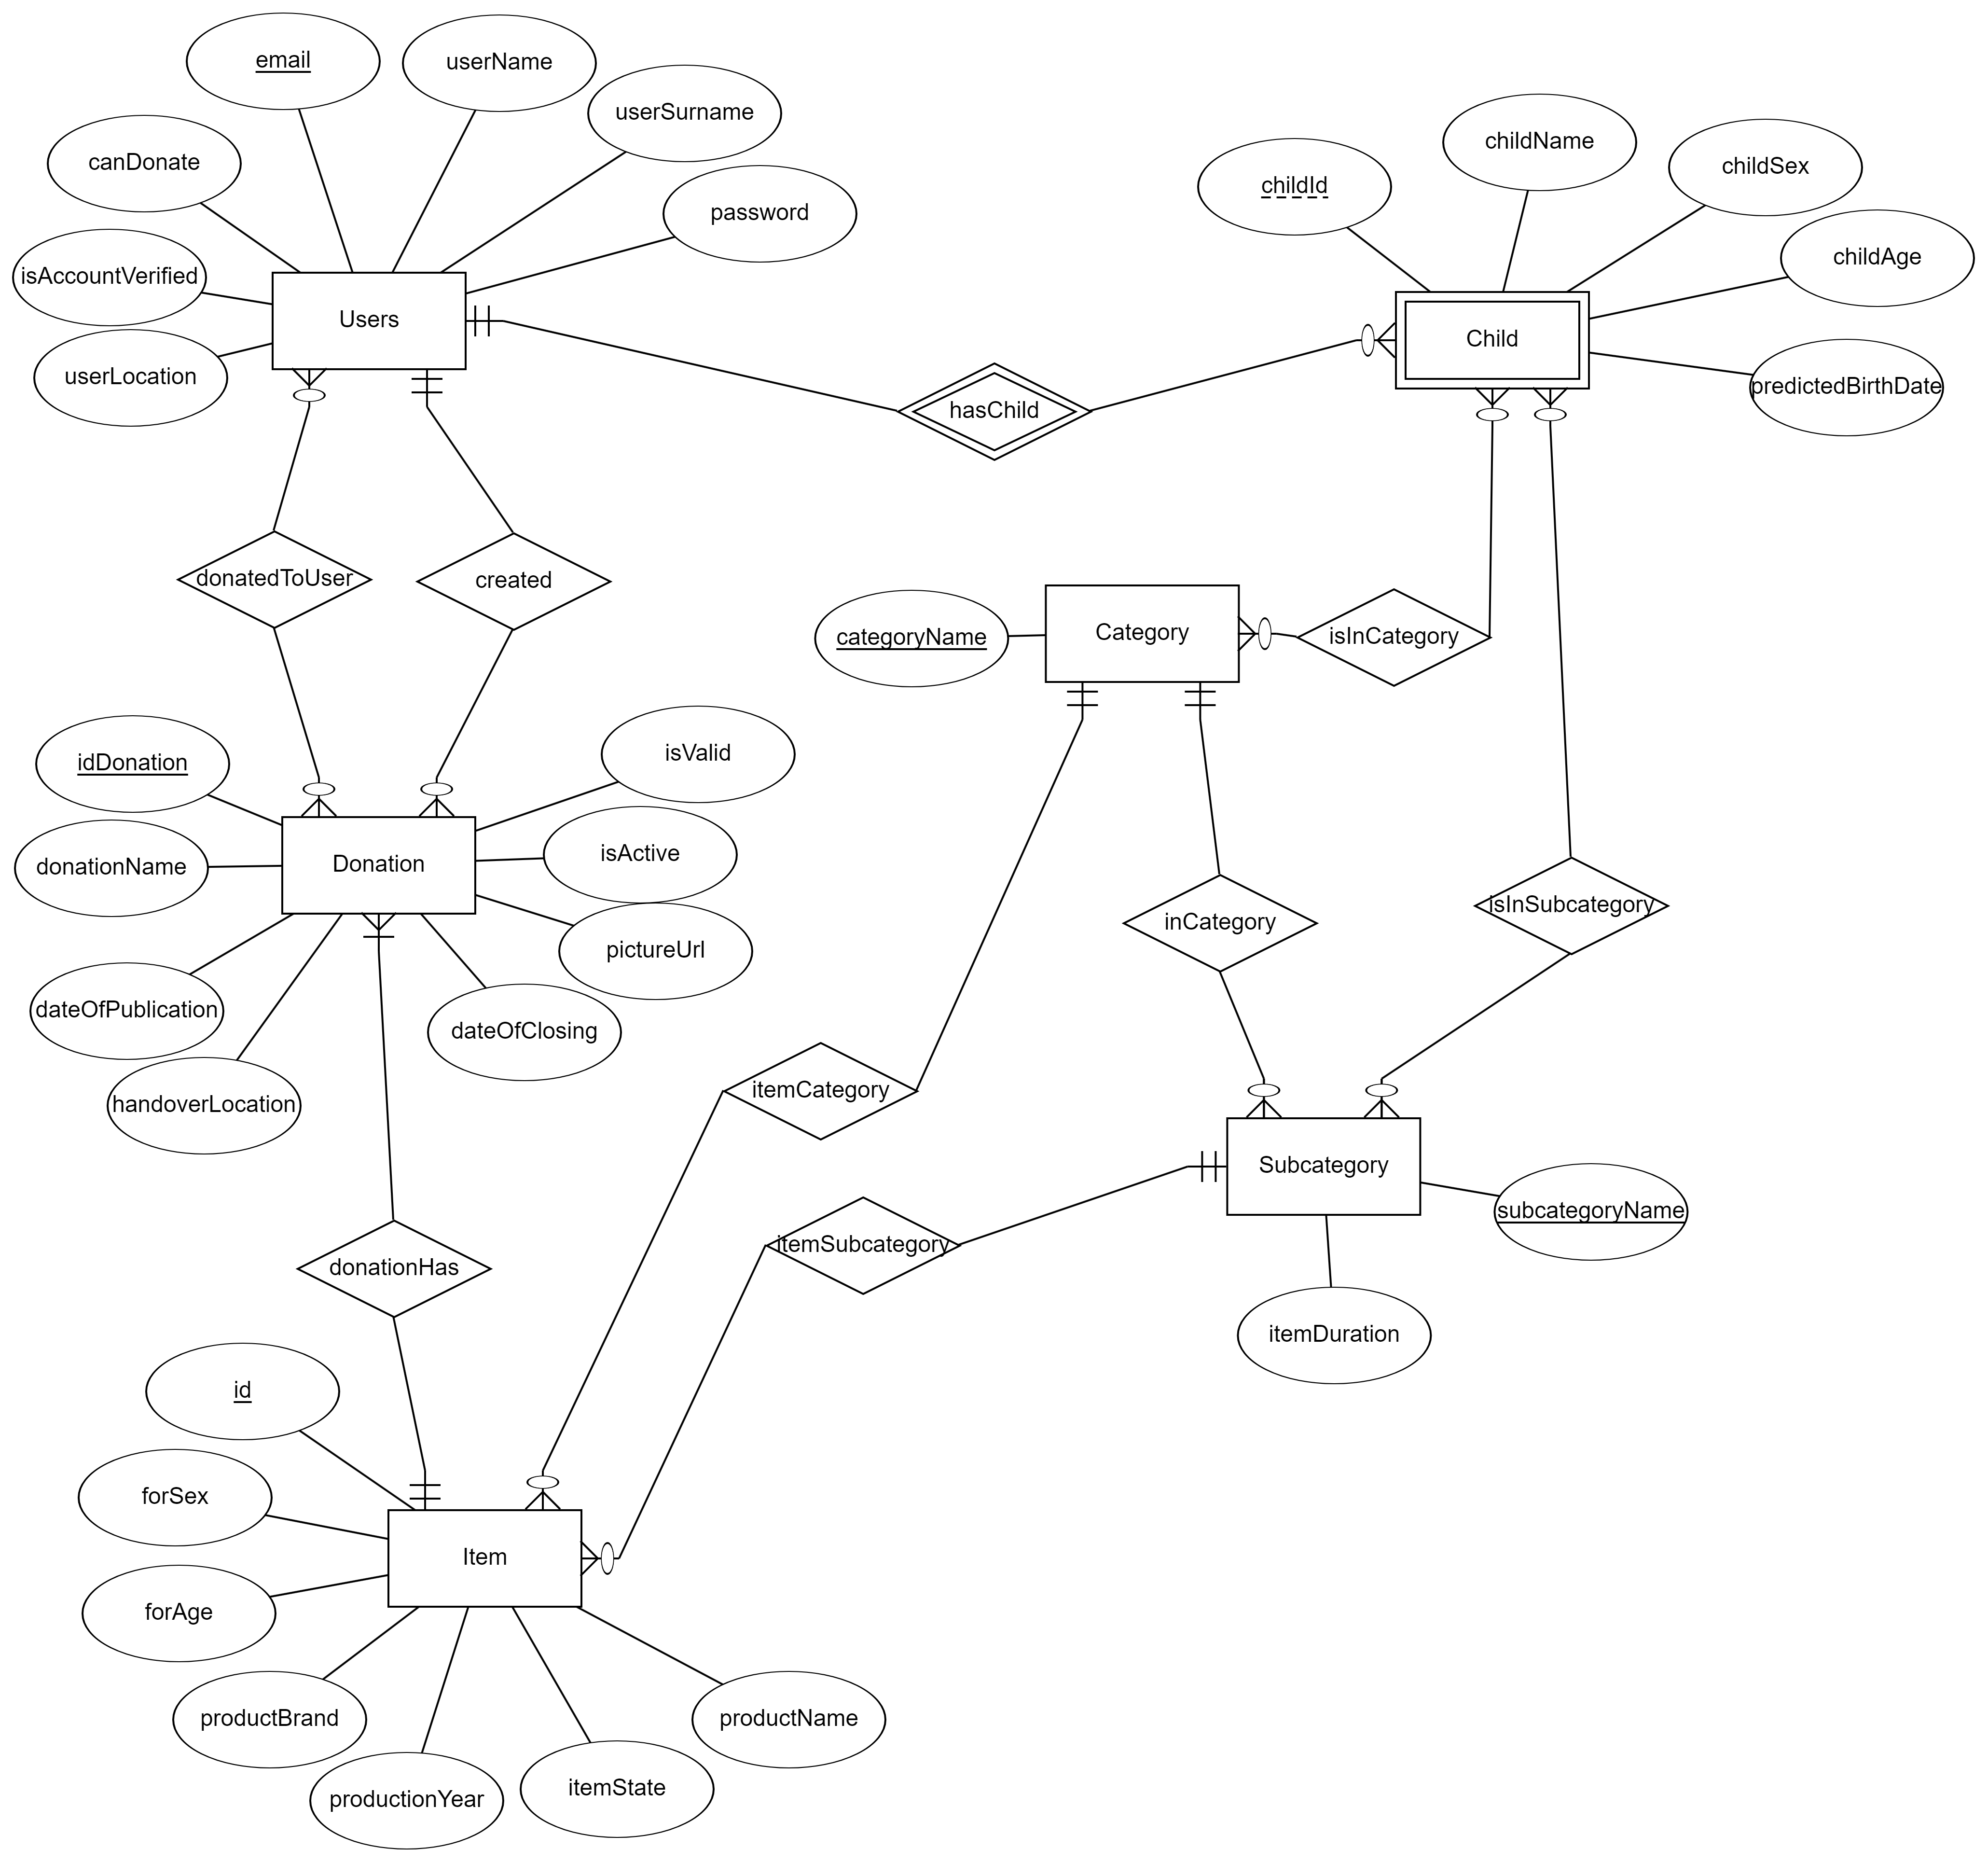
\includegraphics[width=\textwidth,height=0.7\textheight]{dijagrami/ERdijagram.png}
					\centering
					\caption{ER dijagram - aplikacija Djeca za djecu}
					\label{fig:ERDiagram}
				\end{figure}

				\begin{figure}[H]
					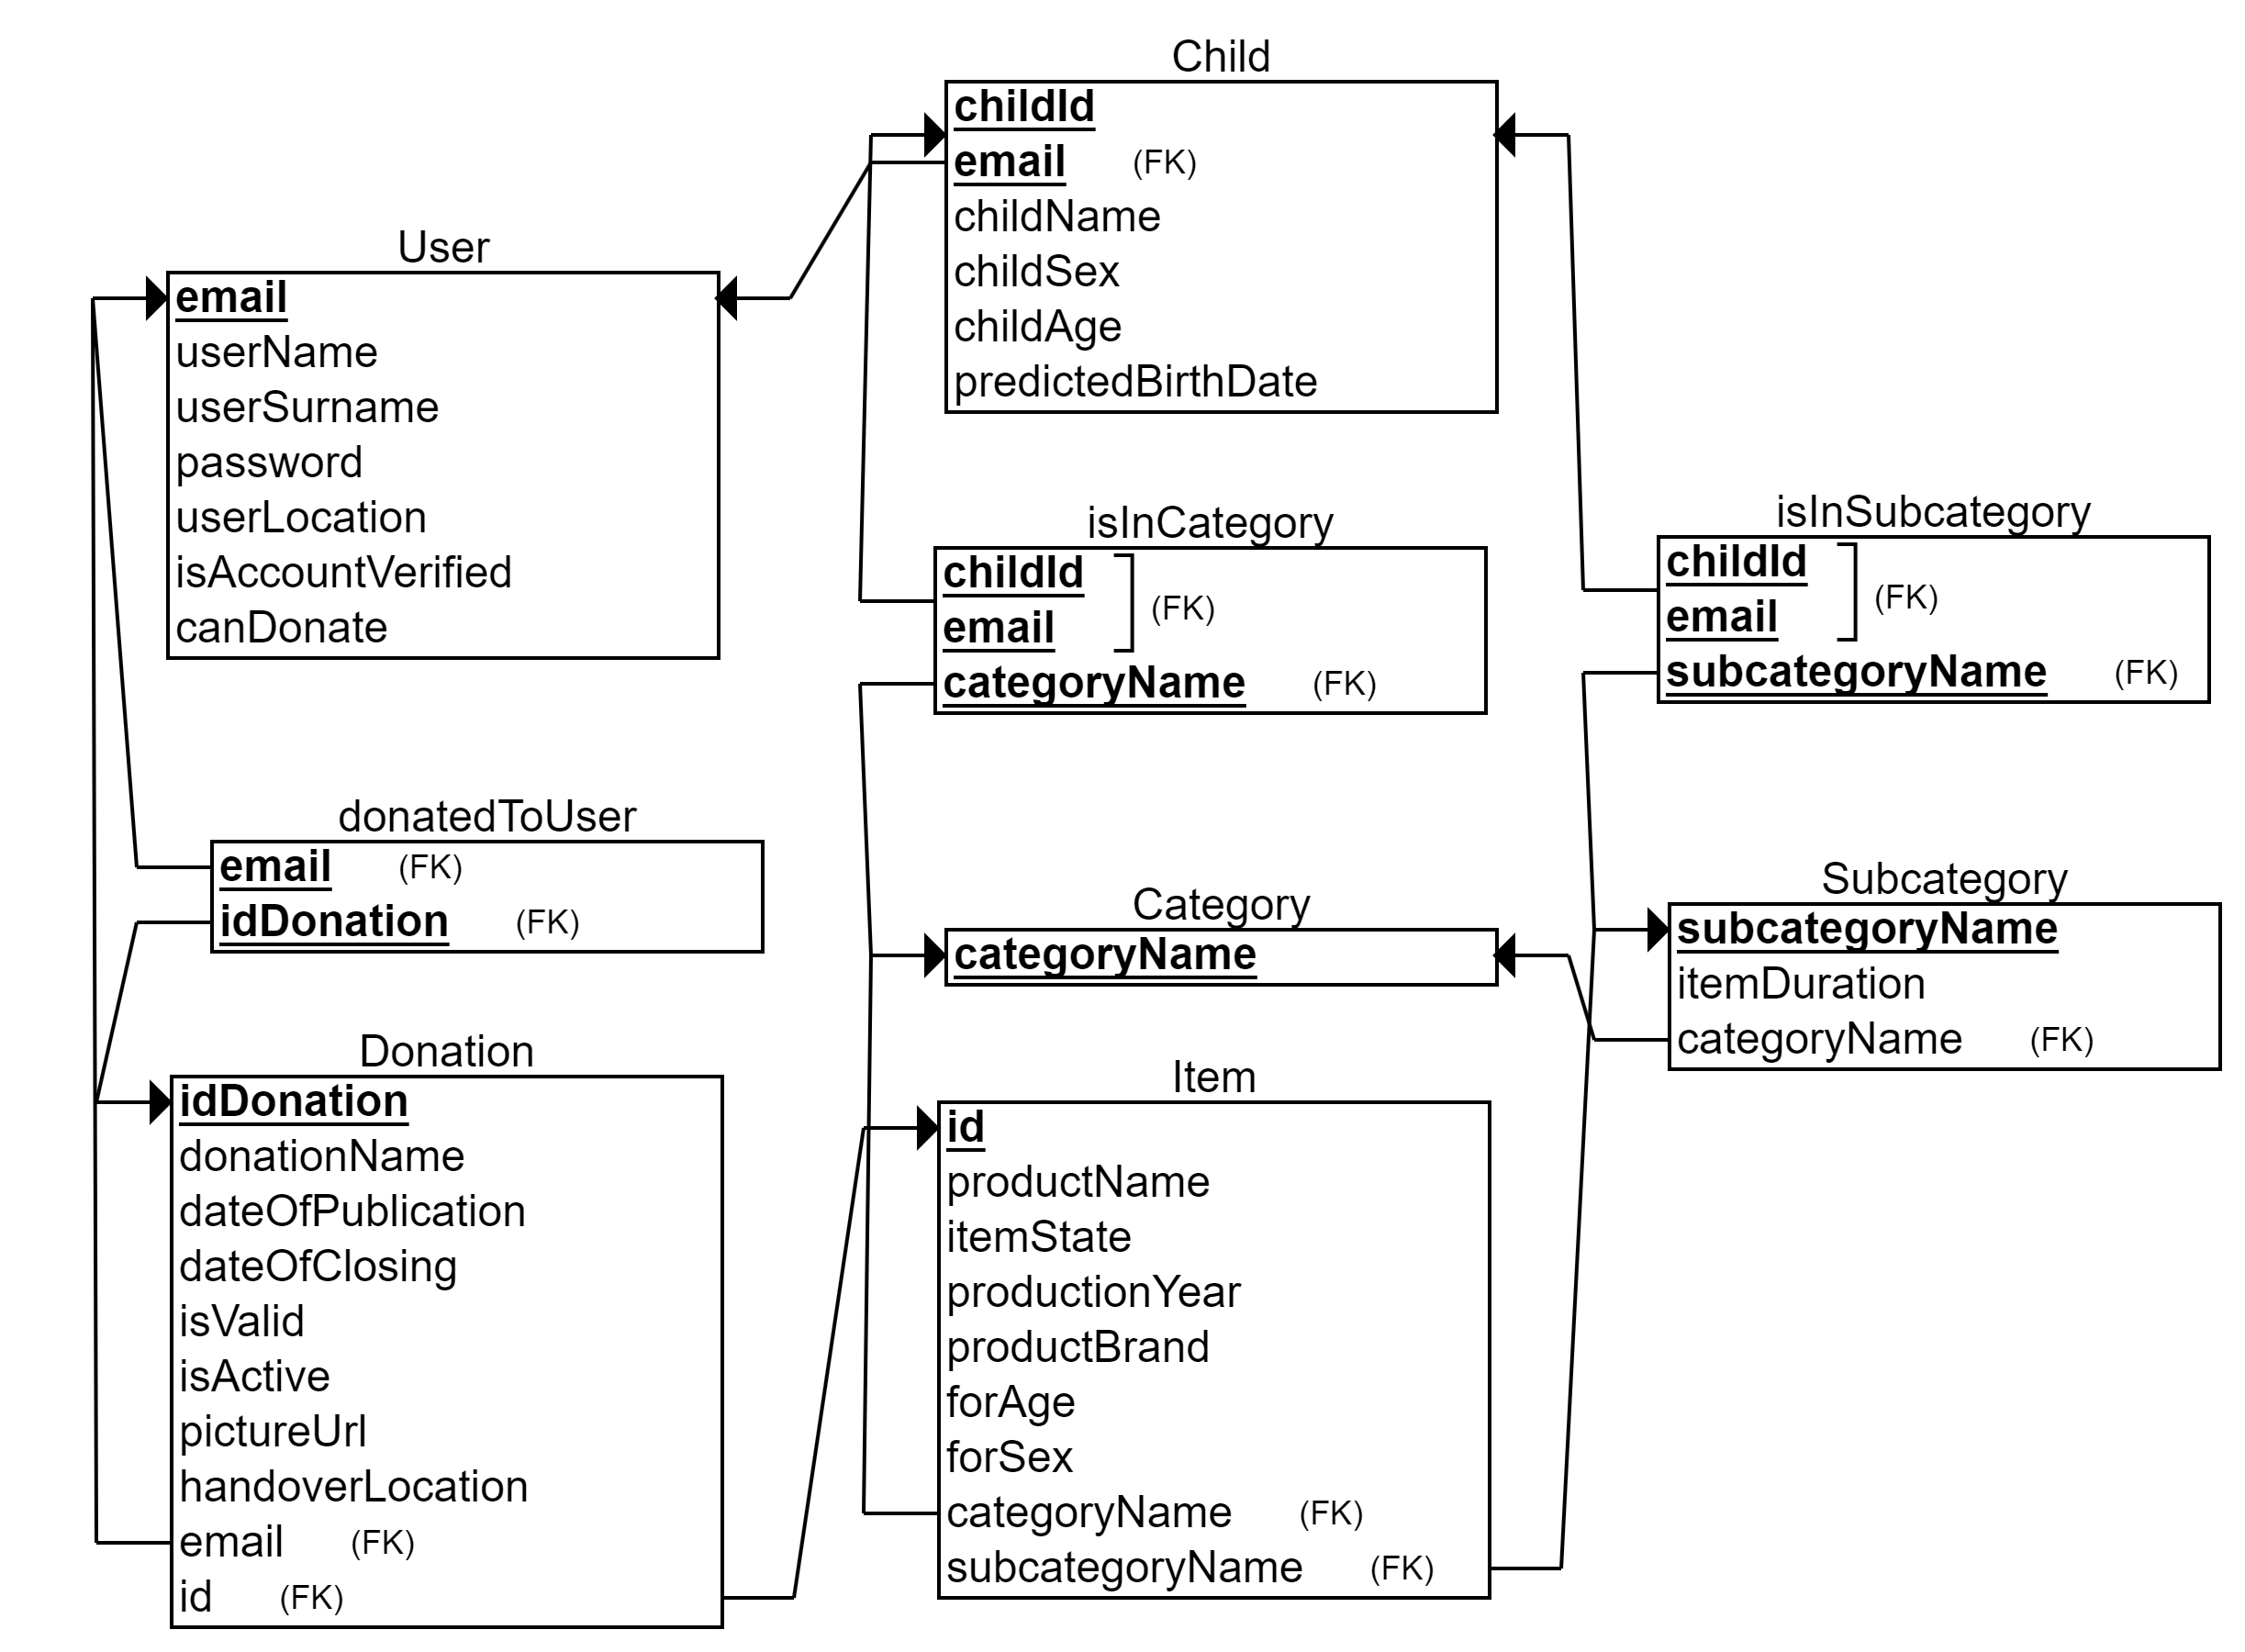
\includegraphics[width=\textwidth,height=0.7\textheight]{dijagrami/RelDijagram.png}
					\centering
					\caption{Relacijski dijagram - aplikacija Djeca za djecu}
					\label{fig:RelDijagram}
				\end{figure}
			\eject
			
			
		\section{Dijagram razreda}
			
			%\textbf{\textit{dio 1. revizije}}\\
			
			%\textit{Prilikom prve predaje projekta, potrebno je priložiti potpuno razrađen dijagram razreda vezan uz \textbf{generičku funkcionalnost} sustava. Ostale funkcionalnosti trebaju biti idejno razrađene u dijagramu sa sljedećim komponentama: nazivi razreda, nazivi metoda i vrste pristupa metodama (npr. javni, zaštićeni), nazivi atributa razreda, veze i odnosi između razreda.}\\
			
			Na slikama 4.4 do 4.7 prikazani su razredi koji pripadaju backend dijelu našeg sustava. U pitanju su specifikacijski dijagrami razreda - implementacijski dijagrami prikazani su nakon opisa specifikacijskih dijagrama.\\[5pt]

			Slika 4.4 prikazuje razrede koji predstavljaju modele - preslikane relacije baze podataka. Razred User predstavlja registriranog korisnika sustava. Razred Child predstavlja dijete registriranog korisnika sustava. Razred Donation predstavlja jednu donaciju zabilježenu u sustavu. 
			Razred Item predstavlja jedan predmet vezan za neke od donacija. Razred Category predstavlja podatke o jednoj od kategorija u koje mogu biti svrstani predmeti. Razred Subcategory predstavlja podatke o jednoj od potkategorija u koje mogu biti svrstani predmeti.\\[10pt]

			\begin{figure}[H]
				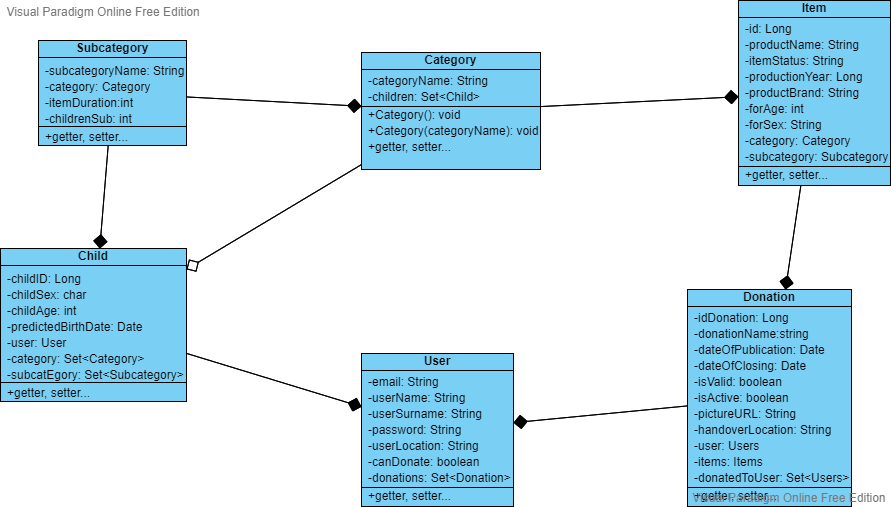
\includegraphics[width=\textwidth,height=0.35\textheight]{dijagrami/Modeli.png}
				\centering
				\caption{Dijagram razreda - dio Models}
				\label{fig:Models}
			\end{figure}
			\eject
			Slika 4.5 prikazuje odnos komponenti na primjeru razreda Category. Razred CategoryController prihvaća i odgovara na HTTP zahtjeve poslane od korisnika tj. konkretnije frontenda. Kako bi na njih ispravno odgovorio, uspostavlja komunikaciju s razredom CategoryServiceJpa.
			Razred CategoryServiceJpa implementira sučelje CategoryService kako bi obavljao potrebne izračune i osigurao uspješno provođenje poslovne logike. Uz to, razred CategoryServiceJpa uspostavlja komunikaciju s razredom CategoryRepository koji služi kao sučelje za pohranu i dohvat podataka iz baze.
			Kako bi prikaz bio što sažetiji, odnos komponenti prikazan je samo na jednom razredu. U stvarnoj implementaciji, ovakav odnos komponenti tj. razreda postoji za svaki razred iz dijela Models.\\[10pt]

			\begin{figure}[H]
				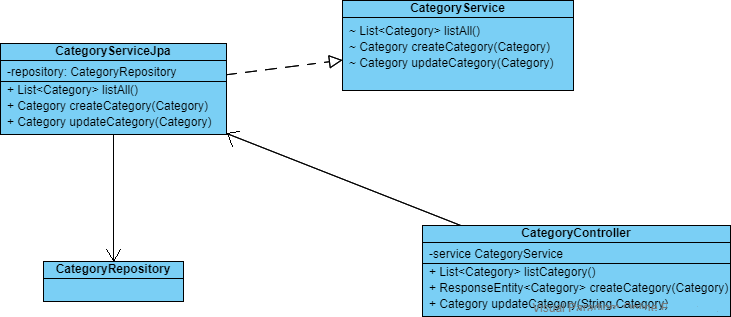
\includegraphics[width=\textwidth,height=0.35\textheight]{dijagrami/OdnosKomponenti.png}
				\centering
				\caption{Dijagram razreda - odnos komponenti}
				\label{fig:OdnosKomponenti}
			\end{figure}

			\eject

			Slika 4.6 prikazuje razrede izvedene iz razreda RestController. Svaki od razreda izvedenih iz RestController služi za prihvaćanje i odgovor na HTTP zahtjeve poslane od strane korisnika tj. konkretnije frontenda.\\[10pt]
			%Razred UsersController služi za slanje odgovora na zahtjeve vezane uz podatke o korisnicima.
			%Razred UsersDetailsService služi za slanje odgovora na zahtjeve vezane uz detaljne podatke o korisnicima.
			%Razred RolesController služi za slanje odgovora na zahtjev vezan uz podatke o ulogama korisnika.
			%Razred ChildController služi za slanje odgovora na zahtjeve vezane uz podatke o djeci.
			%Razred ItemController služi za slanje odgovora na zahtjeve vezane uz podatke o predmetima iz donacija.
			%Razred DonationController služi za slanje odgovora na zahtjeve vezane uz podatke o donacijama.
			%Razred CategoryController služi za slanje odgovora na zahtjeve vezane uz podatke o kategorijama.
			%Razred SubcategoryController služi za slanje odgovora na zahtjeve vezane uz podatke o potkategorijama.\\[10pt]

			\begin{figure}[H]
				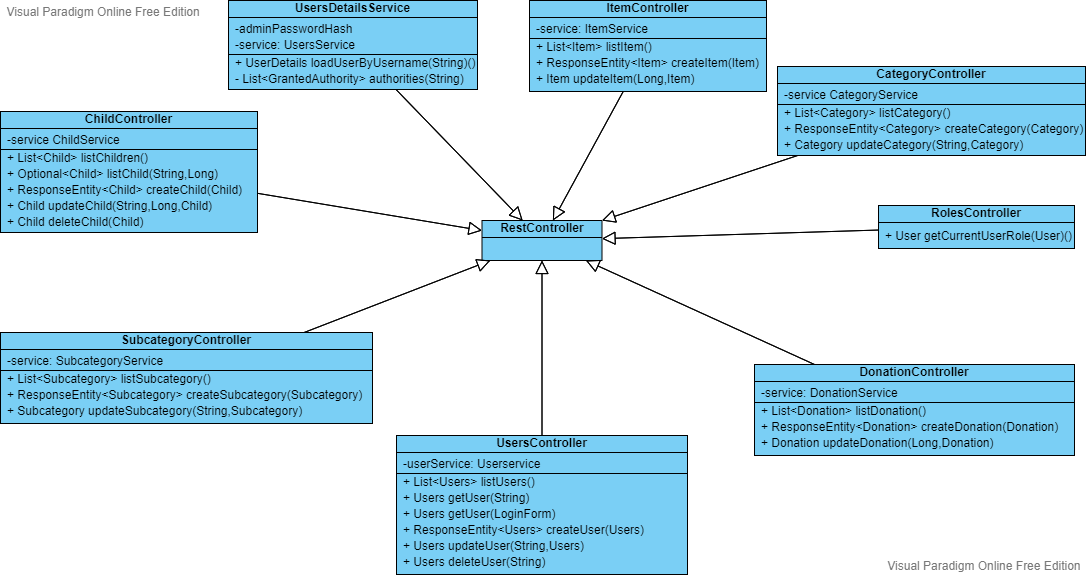
\includegraphics[width=\textwidth,height=0.4\textheight]{dijagrami/Controlleri.png}
				\centering
				\caption{Dijagram razreda - dio Controllers}
				\label{fig:Controllers}
			\end{figure}

			\eject

			Slika 4.7 prikazuje razrede izvedene iz razreda JpaRepository. Svaki od prikazanih razreda služi kao sučelje za pohranu i dohvat podataka iz baze podataka za svoju pripadajuću relaciju.\\[10pt]

			\begin{figure}[H]
				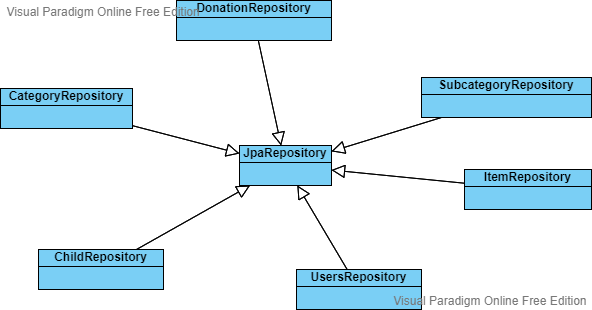
\includegraphics[width=\textwidth,height=0.4\textheight]{dijagrami/Repozitoriji.png}
				\centering
				\caption{Dijagram razreda - dio Repositories}
				\label{fig:Repositories}
			\end{figure}

			%\textbf{\textit{dio 2. revizije}}\\

                Na slikama 4.8 - 4.15 prikazani su implementacijski dijagrami razreda generirani direktno iz koda. Uz dijagrame razreda za koje su već opisani specifikacijski dijagrami (Models, odnos komponenti, Controllers, Repositories) dodatno su uključeni i dijagram razreda koji prikazuje odnos između UsersController klase i EmailSenderService klase koja se koristi za slanje potvrde o registraciji korisnika na mail, kao i dijagram razreda koji prikazuje odnos klasa za ostvarenje sigurnosti, autentifikacije i autorizacije korisnika. Zbog preglednosti dijagrami razreda za dio Controllers i dio Repositories podijeljeni su u dva dijela.
			
			\eject

                \begin{figure}[H]
				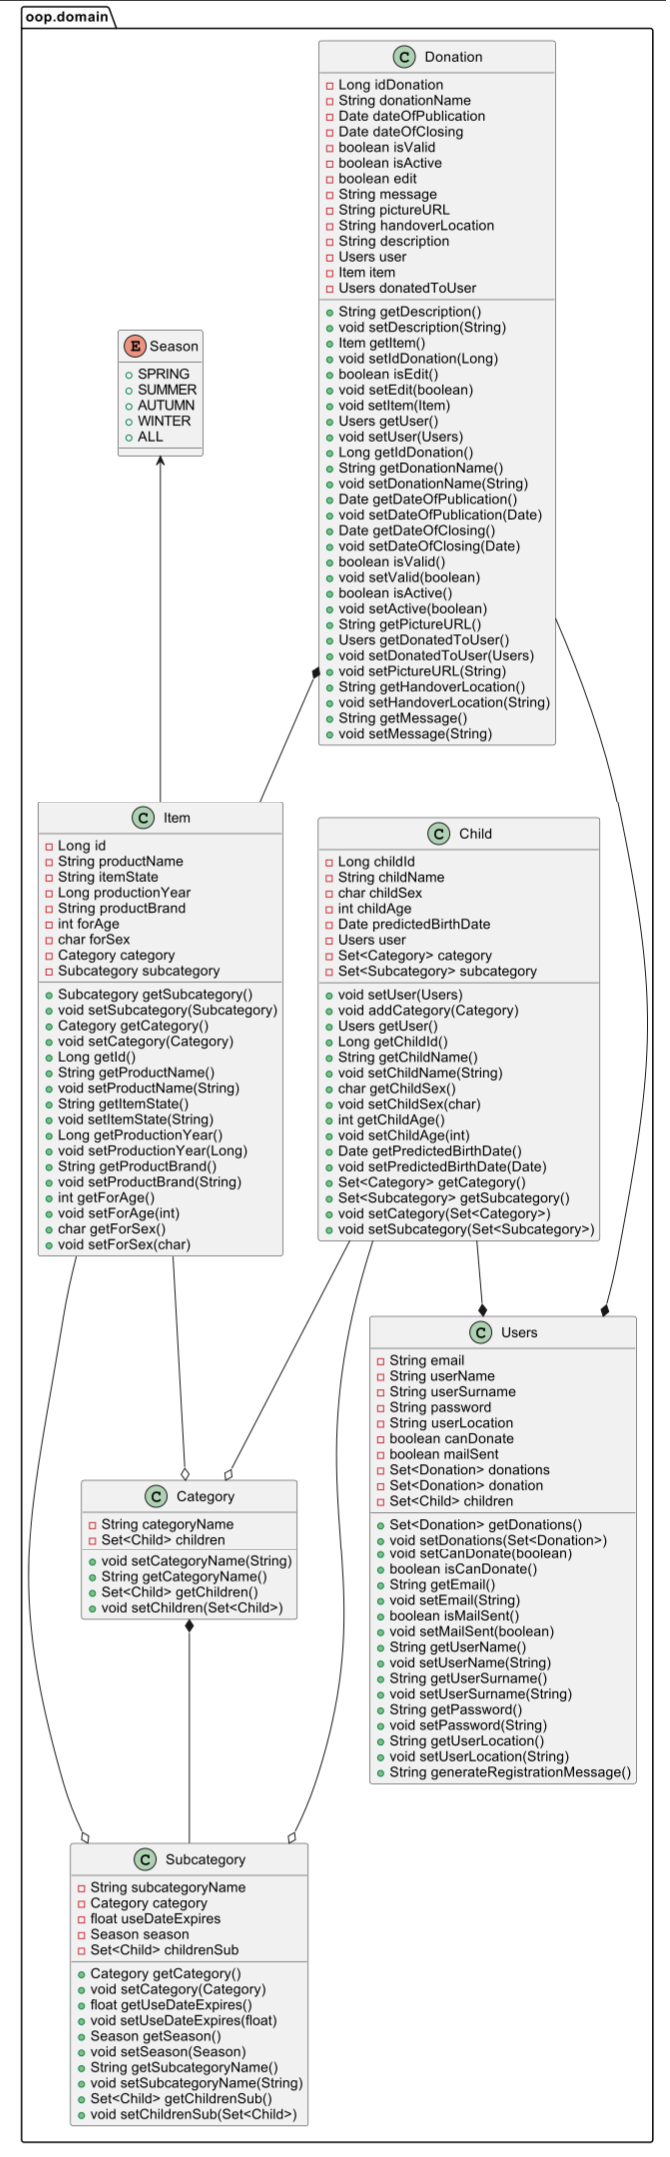
\includegraphics[width=\textwidth,height=0.95\textheight]{dijagrami/Modeli Final.png}
				\centering
				\caption{Dijagram razreda - dio Models (finalna verzija)}
				\label{fig:ModelsFinal}
			\end{figure}

                \begin{figure}[H]
				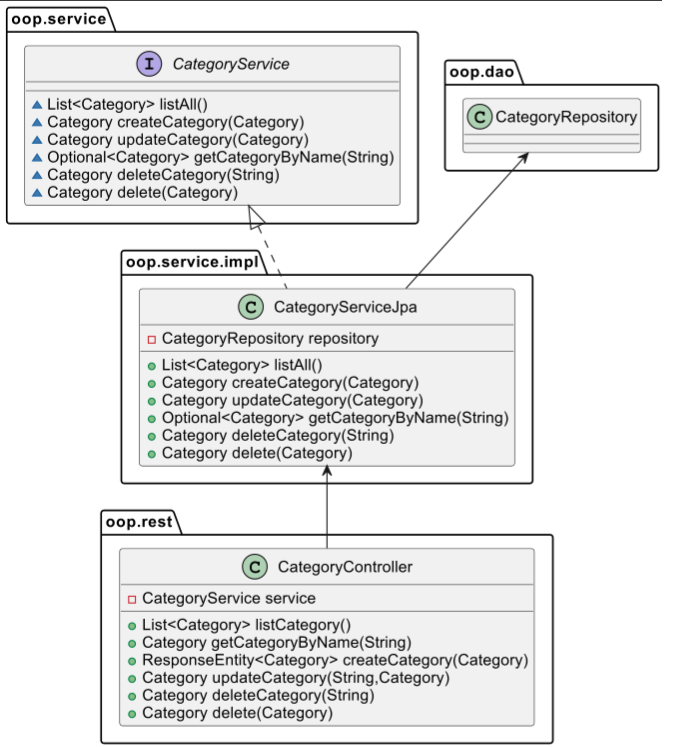
\includegraphics[width=\textwidth,height=0.8\textheight]{dijagrami/Odnos komponenti Final.png}
				\centering
				\caption{Dijagram razreda - odnos komponenti (finalna verzija)}
				\label{fig:OdnosKomponentiFinal}
			\end{figure}

                %   \begin{figure}[H]
                %   \makebox[\textwidth][c]{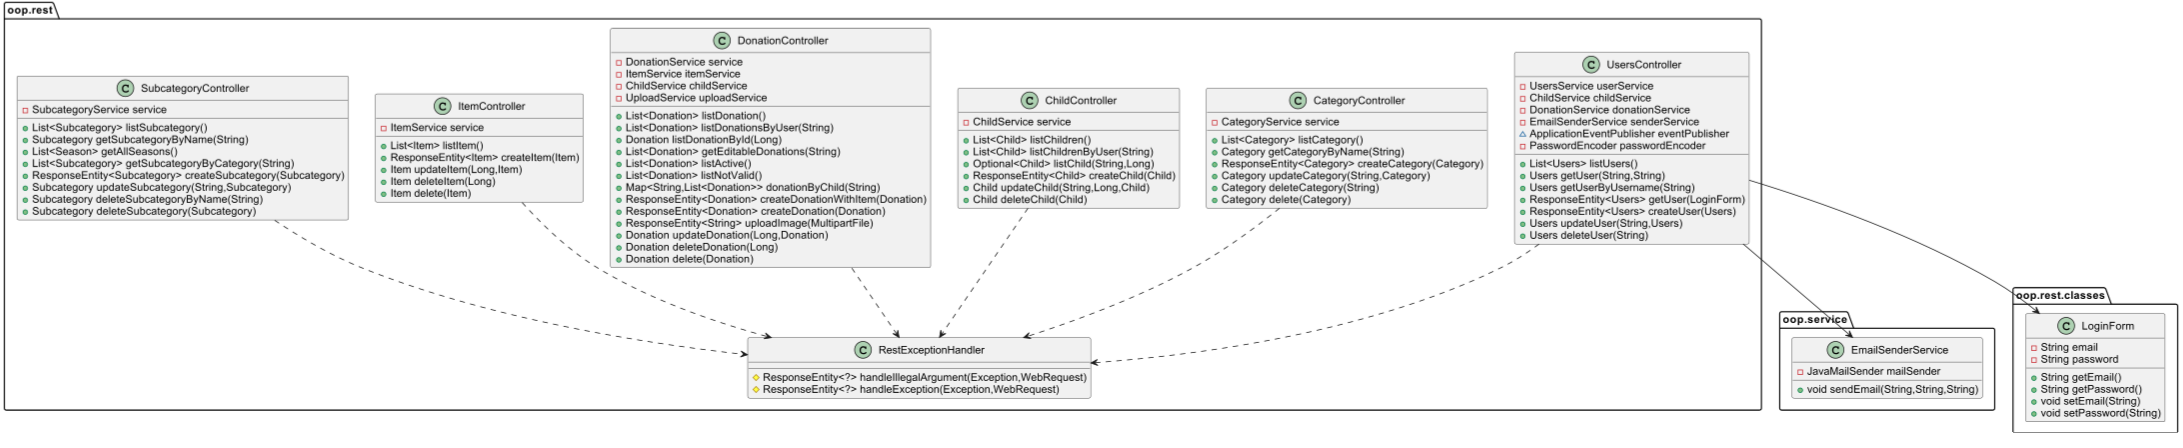
\includegraphics[width=1.3\textwidth,height=0.6\textheight]{dijagrami/Controlleri Final.png}}%
			% 	\centering
			% 	\caption{Dijagram razreda - dio Controllers (finalna verzija)}
			% 	\label{fig:ControllersFinal}
			% \end{figure}

                \begin{figure}[H]
				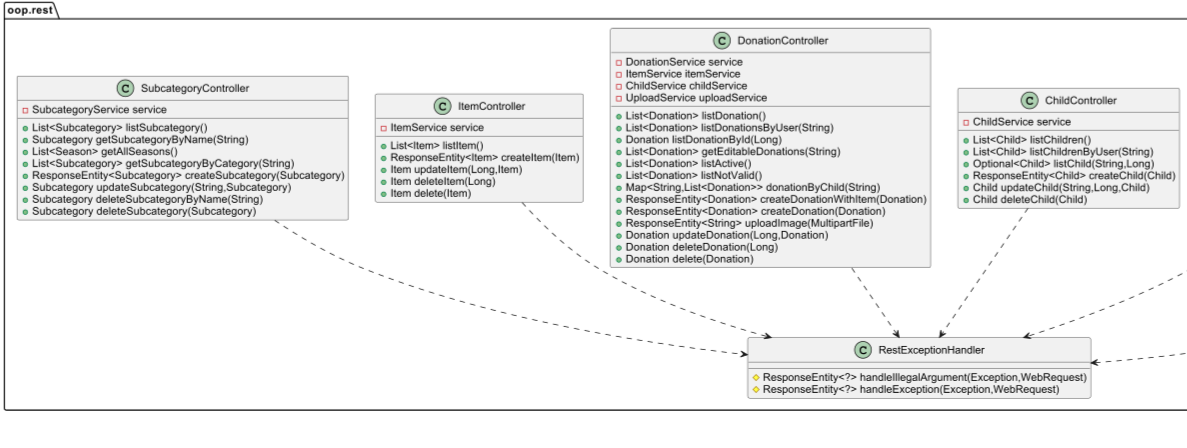
\includegraphics[width=\textwidth,height=0.4\textheight]{dijagrami/Controlleri Final Part1.png}
				\centering
				\caption{Dijagram razreda - dio Controllers, prvi dio (finalna verzija)}
				\label{fig:ControllersFinalPt1}
			\end{figure}

                \begin{figure}[H]
				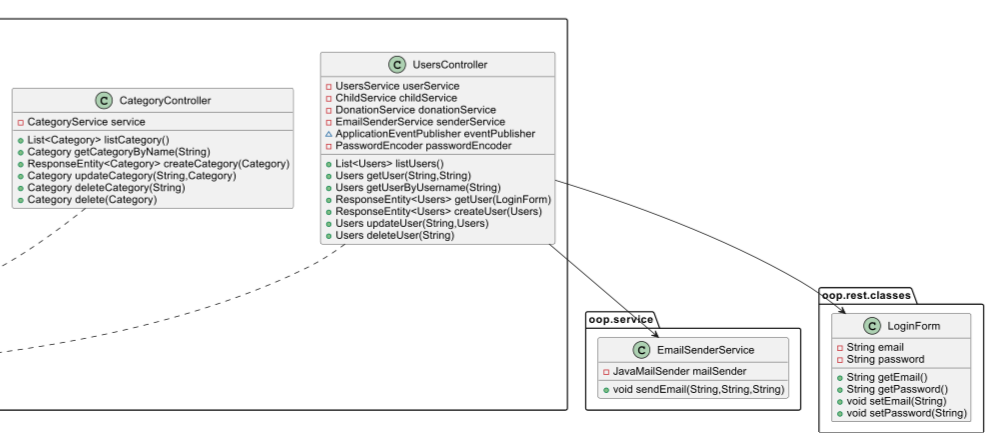
\includegraphics[width=\textwidth,height=0.4\textheight]{dijagrami/Controlleri Final Part2.png}
				\centering
				\caption{Dijagram razreda - dio Controllers, drugi dio (finalna verzija)}
				\label{fig:ControllersFinalPt2}
			\end{figure}

                \begin{figure}[H]
                \makebox[\textwidth][c]{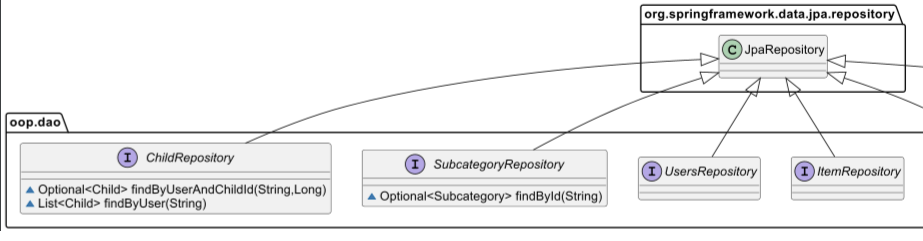
\includegraphics[width=1.2\textwidth,height=0.4\textheight]{dijagrami/Repozitoriji Final Part1.png}}%
				\centering
				\caption{Dijagram razreda - dio Repositories, prvi dio (finalna verzija)}
				\label{fig:RepositoriesFinalPt1}
			\end{figure}

                \begin{figure}[H]
				\makebox[\textwidth][c]{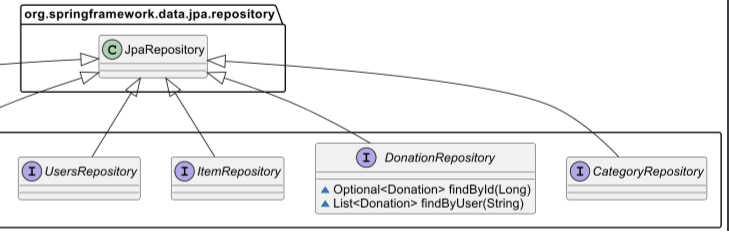
\includegraphics[width=1.2\textwidth,height=0.4\textheight]{dijagrami/Repozitoriji Final Part2.png}}%
				\centering
				\caption{Dijagram razreda - dio Repositories, drugi dio (finalna verzija)}
				\label{fig:RepositoriesFinalPt2}
			\end{figure}

                \begin{figure}[H]
				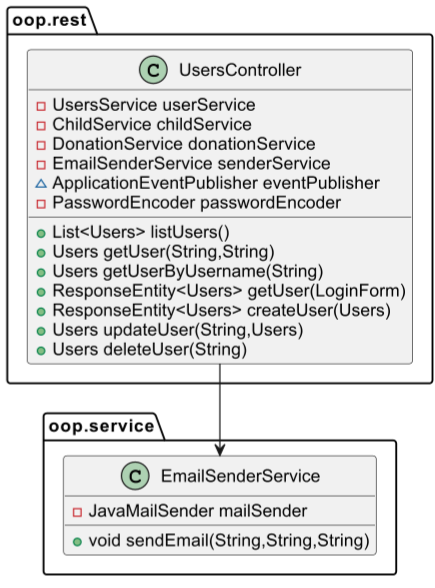
\includegraphics[width=\textwidth,height=0.4\textheight]{dijagrami/EmailService.png}
				\centering
				\caption{Dijagram razreda - dio Email Service}
				\label{fig:EmailService}
			\end{figure}

                \begin{figure}[H]
				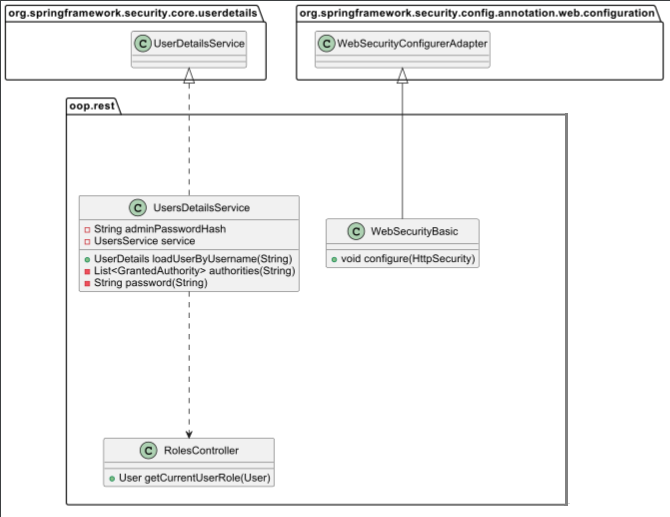
\includegraphics[width=\textwidth,height=0.4\textheight]{dijagrami/Security.png}
				\centering
				\caption{Dijagram razreda - dio Security}
				\label{fig:Security}
			\end{figure}
   
			\eject
		
		\section{Dijagram stanja}
			
                Dijagram stanja prikazan na slici 4.16 prikazuje stanja u kojima se može naći sustav (konkretno, u pitanju je korisničko sučelje - frontend), kao i prijelaze pomoću kojih sustav dolazi u druga stanja. Svaki prijelaz označen je događajem (npr. "Klik na proizvoljni oglas"), kao i akcijom (npr. "Prikaži aktivne oglase()") koja se izvršava "tijekom prijelaza" - nakon što se dogodio događaj koji je potaknuo prijelaz u drugo stanje. Većina akcija označenih na prijelazima isto tako mogla je biti označena kao entry odnosno exit akcija samoga stanja, ali je zbog preglednosti i konzistentnosti odabran prikaz takvih akcija na prijelazima. Dijagram na slici 4.16 prikazuje stanja u kojima se sustav može naći kada je u sustav ulogiran registrirani korisnik za kojeg je administrator stavio dopuštenje da može donirati - da korisnik nema dopuštenje, sustav se pri radu s takvim korisnikom ne bi mogao naći u stanju "Kreiranje oglasa", kao ni u stanju "Korisnikove donacije" jer ono služi za prikaz korisnikovih prijašnjih, kao i trenutnih donacija. \\

                \begin{figure}[H]
				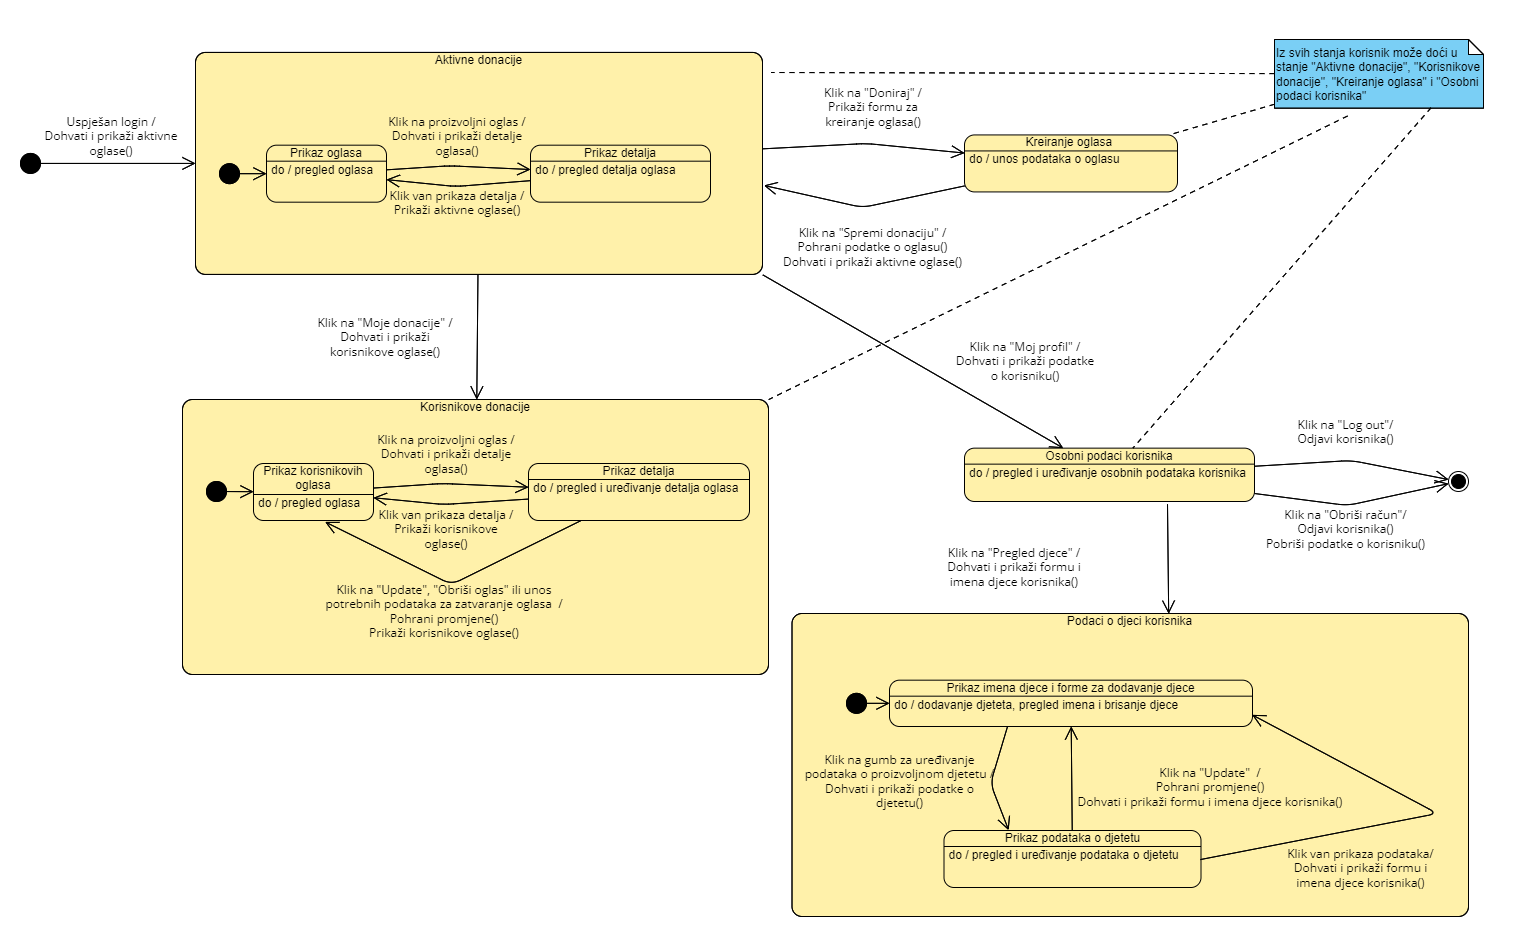
\includegraphics[width=\textwidth,height=0.45\textheight]{dijagrami/Dijagram stanja.png}
				\centering
				\caption{Dijagram stanja}
				\label{fig:StateDiagram}
			\end{figure}
			
			\eject 
                
                Kako bi napravili razliku između akcija koje izvršava sustav i akcija koje radi korisnik u interakciji sa sustavom, sve akcije koje izvršava sustav na kraju imaju oznaku () (slično pozivu funkcije u kodu). Radi preglednosti, neke od strelica nisu prikazane na dijagramu - korisnik iz bilo kojeg stanja može preći u stanje "Aktivne donacije", "Korisnikove donacije", "Kreiranje oglasa" i "Osobno podaci korisnika" jer je prijelaz u ta stanja ostvaren klikom na odgovarajući dio zaglavlja stranice. Akcije koje radi korisnik u interakciji u sustavu naznačene su kao do akcije unutar stanja ili kao događaji koji potiču prijelaze u druga stanja.\\
                                
			Nakon uspješnog logina, registrirani korisnik preusmjeren je na stranicu Aktivne donacije na kojoj može pregledavati sve oglase, ali isto tako i pregledavati detalje proizvoljnih oglasa. Pomoću zaglavlja stranice korisnik može doći do stranice Aktivne donacije, stranice za kreiranje oglasa, stranice za prikaz i uređivanje osobnih podataka te stranice za prikaz vlastitih donacija. Na stranici za kreiranje oglasa korisnik unosi podatke i nakon unosa klikom na gumb "Spremi donaciju" biva preusmjeren na stranicu za prikaz vlastitih donacija. Na stranici za prikaz vlastitih donacija korisnik može pregledavati sve oglase koje je sam kreirao ili zaprimio, kao i detalje o istima. Na stranici za prikaz i uređivanje osobnih podataka korisnik se također može i odjaviti, obrisati svoj račun i otići na stranicu za dodavanje, brisanje i prikaz podataka o djeci. Rad s aplikacijom završava kada korisnik odabere opciju "Log out".
			%\textbf{\textit{dio 2. revizije}}\\

                \eject
                %\textbf{V2}

                %Dijagram stanja prikazan na slici 4.9 prikazuje stanja u kojima se može naći sustav (konkretno, u pitanju je korisničko sučelje - frontend), kao i prijelaze pomoću kojih sustav dolazi u druga stanja. Svaki prijelaz označen je događajem (npr. "Klik na proizvoljni oglas"), a po potrebi i uvjetom (u uglatim zagradama). \\

                %\begin{figure}[H]
                %\makebox[\textwidth][c]{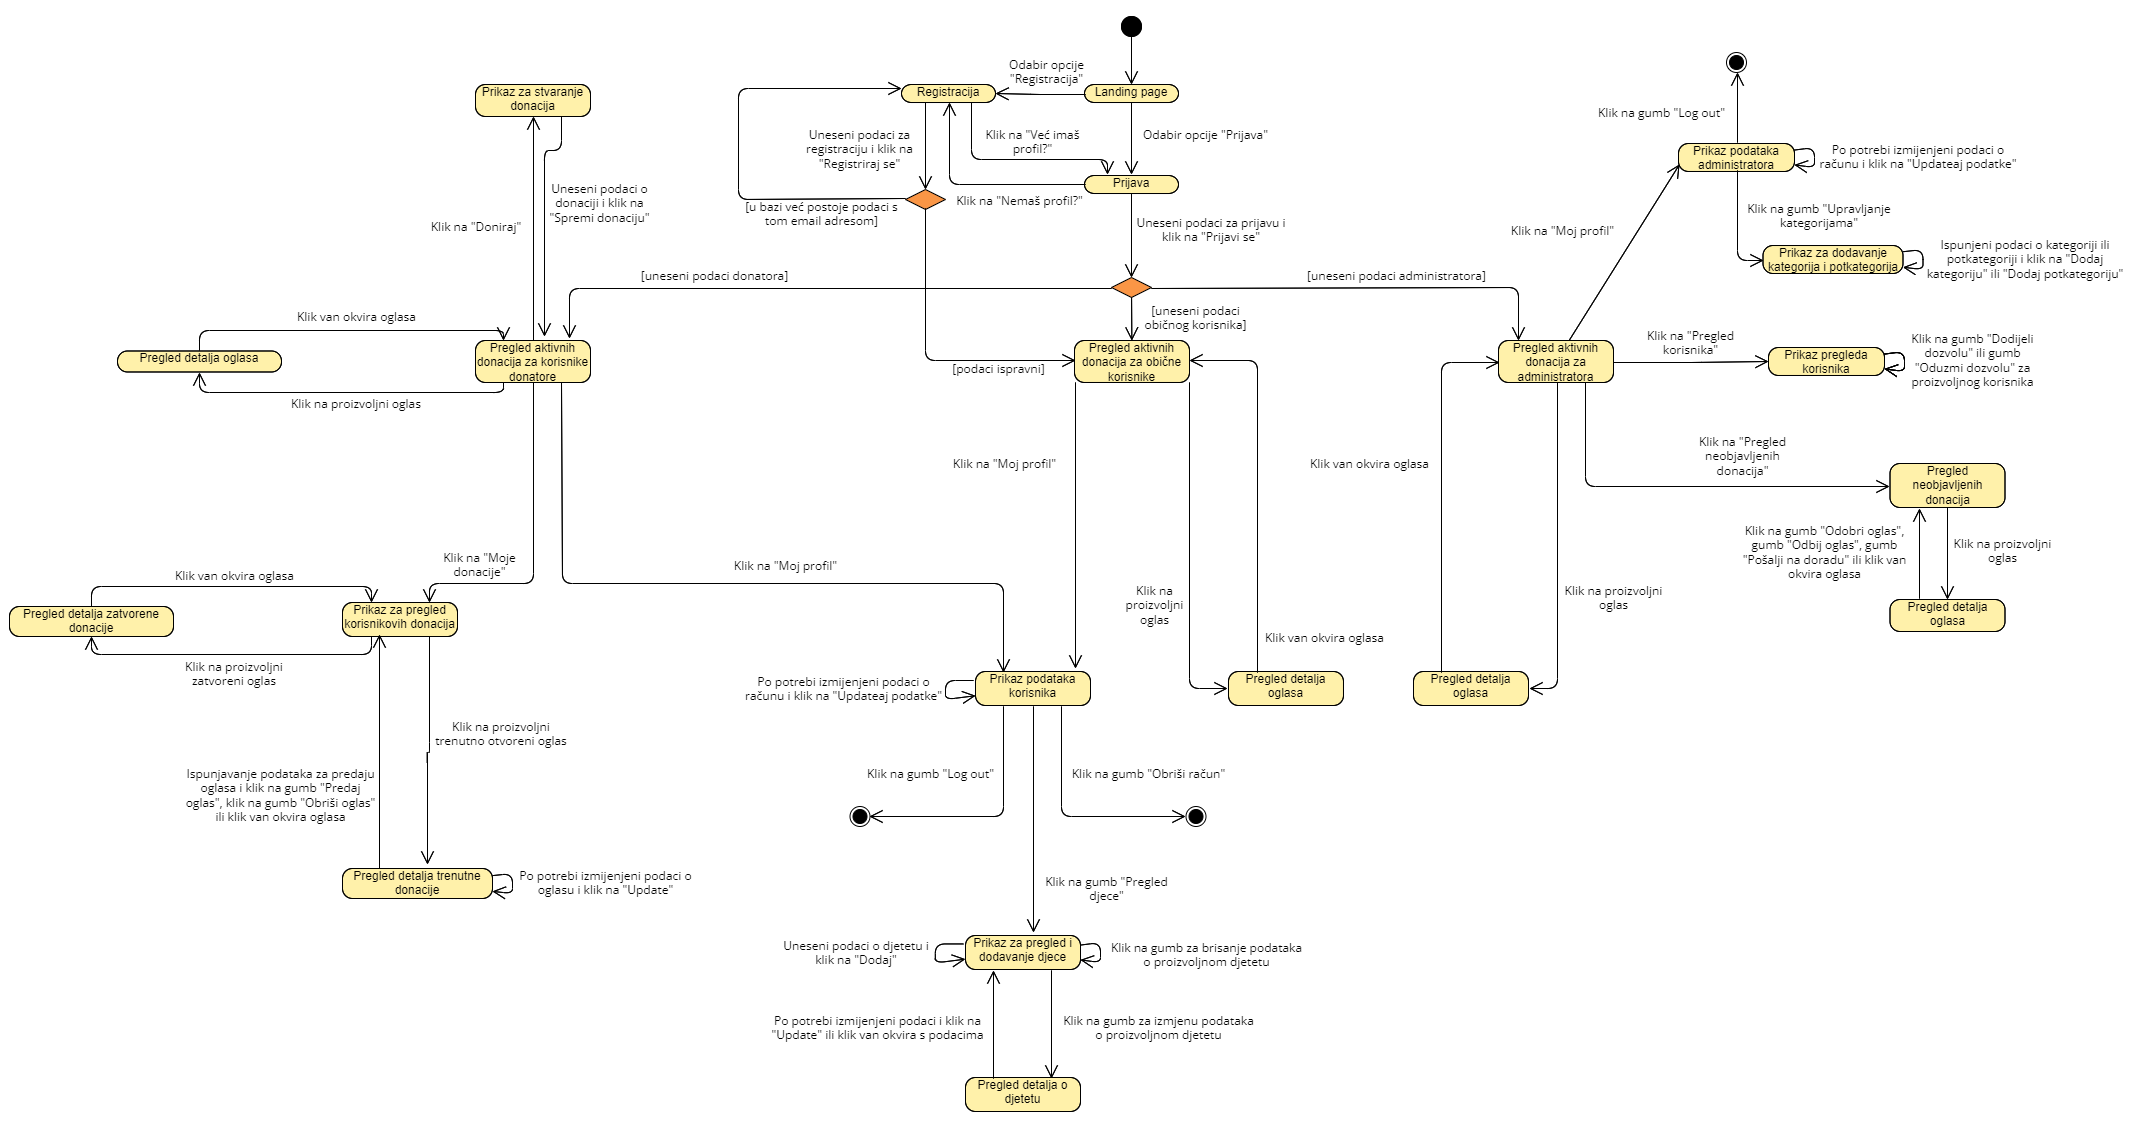
\includegraphics[scale=0.35]{dijagrami/Dijagram stanja v2.png}}%
				%\centering
				%\caption{Dijagram stanja, druga inačica}
				%\label{fig:StateDiagramv2}
			%\end{figure}
                 %Ovisno o tome koja je razina prava dodijeljena korisniku s unešenim podacima, nakon uspješnog logina korisniku se prikaže jedna od tri moguće stranice. Stranice se razlikuju u izgledu svoga zaglavlja (engl. page header) - administrator ima opcije pregledavati aktivne oglase, pregledavati i odobravati neobjavljene oglase, pregledavati popis korisnika i dodijeljivati im pravo za doniranje, ali i pregledavati i mijenjati svoje podatke. S druge strane, običan korisnik ima pravo samo pregledavati aktivne oglase i pregledavati i mijenjati vlastite podatke, pritom dodajući, brišući ili izmjenjujući podatke o svojoj djeci. Donator uz mogućnosti običnog korisnika može i stvarati oglase te pregledavati svoje do sada objavljene oglase, bilo da je u pitanju već zatvoren oglas ili trenutno otvoreni oglas - trenutno otvorene oglase donatori mogu urediti, obrisati ili zatvoriti. \\
                 
                 %Radi preglednosti, neke od strelica nisu prikazane na dijagramu - običan korisnik iz bilo kojeg stanja može preći u stanje "Prikaz aktivnih donacija za obične korisnike" i  "Prikaz podataka korisnika". Donator uz prijelaz u navedena stanja ("Pregled aktivnih donacija za korisnike donatore", "Prikaz podataka korisnika") može iz bilo kojeg stanja prijeći i u stanja "Prikaz za pregled korisnikovih donacija" i "Prikaz za stvaranja donacija", a administrator može iz bilo kojeg stanja prijeći u jedno od sljedećih stanja: "Pregled aktivnih donacija za administratora", "Prikaz podataka administratora", "Prikaz pregleda korisnika", "Pregled neobjavljenih donacija" i "Pregled aktivnih donacija za administratora". Prijelazi u stanja navedena u ovome odlomku ostvareni su klikom na prikladne dijelove zaglavlja stranice, a sama zaglavlja razlikuju se ovisno o razini ovlasti korisnika.\\

                 %Radi preglednosti, nakon klika na gumb "Log out" ili "Obriši račun" sustav ide u završno stanje - u stvarnosti time samo završava trenutna sesija korištenja sustava te se korisniku prikazuje landing page, ali bi dodavanjem strelica za prijelaz u stanje "Landing page" iz potrebnih stanja bila narušena preglednost dijagrama. Akcije sustava (npr. prikaziOglase()) zbog preglednosti također su izostavljena iz dijagrama, time na dijagramu ostavljajući samo korisničke akcije kao događaje koji potiču prijelaz iz jednog stanja sustava u drugo. Isto tako, provjere ispravnosti podataka (npr. provjera jesu li izmijenjeni podaci o korisniku i dalje važeći) izostavljene su iz dijagrama - za svaku provjeru bilo bi potrebno uvesti grananje gdje bi ovisno o ispravnosti podataka sustav ponovno došao u prethodno stanje ili mogao dalje napredovati. 

                %\eject
				
				


		\section{Dijagram aktivnosti}

		Dijagram aktivnosti na jednostavan način prikazuje opis modela toka upravljanja. Na slikama 4.17 i 4.18 su prikazani dijagrami aktivnosti za odabrane procese: proces kreiranja oglasa i proces kreiranja korisničkog računa. \\
			

			 \begin{figure}[H]
                			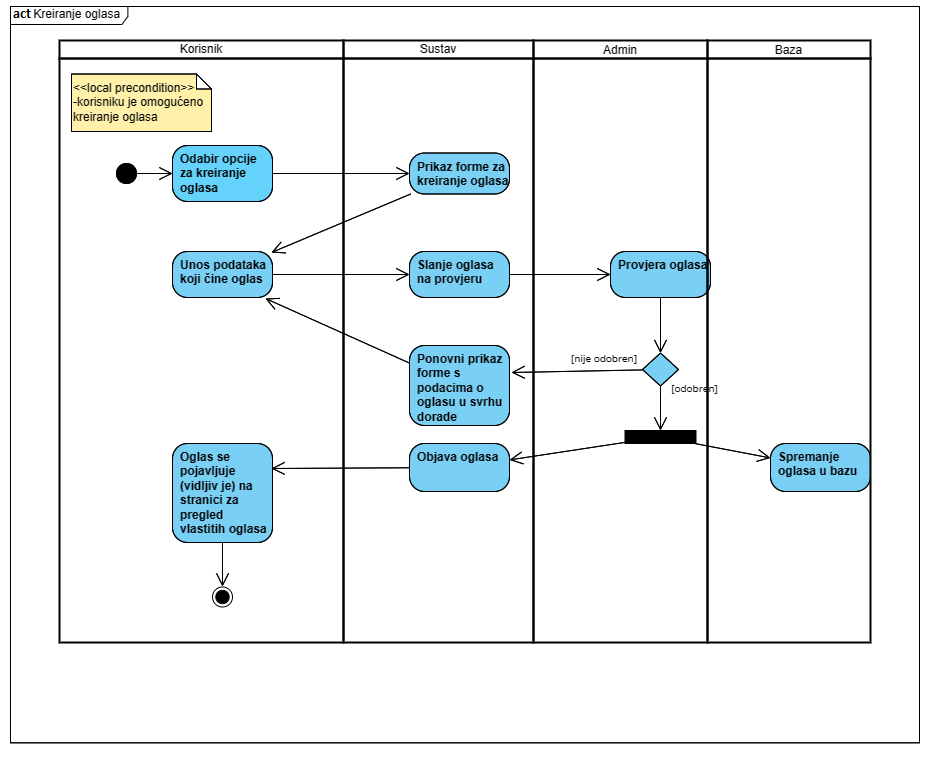
\includegraphics[width=\textwidth,height=0.5\textheight]{dijagrami/DijagramAktivnosti1.png}%
				\centering
				\caption{Dijagram aktivnosti - proces kreiranja oglasa}
				\label{fig:ActivityDiagram1}
			\end{figure}

		Na dijagramu jasno možemo razabrati aktore prema particijama i razlučiti njihove aktivnosti. Vidljivo je da započinjemo s korisnikom koji odabire opciju za kreiranje oglasa. Uvjet da bi uopće mogao izabrati tu opciju jest da mu je objavljivanje/kreiranje oglasa dozvoljeno. Nakon što korisnik izabere opciju slijedi akcija od sustava koji će prikazati formu za kreiranje novog oglasa. Potom korisnik unosi podatke i tako kreira oglas koji zatim sustav šalje na provjeru. Oglase provjerava administrator i može odlučiti sadrži li oglas sve potrebne informacije ili ne i na temelju toga ih odobrava ili ne. Ukoliko oglasi nisu odobreni sustav će ih poslati korisniku na doradu. Odobreni oglasi se, pak objavljuju i spremaju u bazu. Nakon objavljivanja korisniku se njegov oglas pojavljuje na stranici za pregled vlastitih oglasa i time završava proces kreiranja oglasa. \\
			\eject

			
			 \begin{figure}[H]
               			 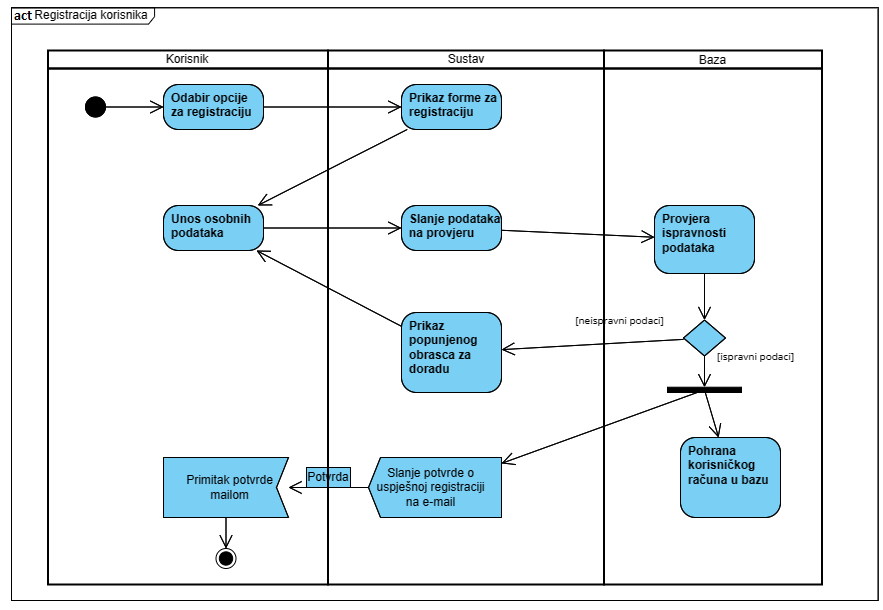
\includegraphics[width=\textwidth,height=0.5\textheight]{dijagrami/DijagramAktivnosti2.png}%
				\centering
				\caption{Dijagram aktivnosti - registracija korisnika}
				\label{fig:ActivityDiagram2}
			\end{figure}

		Na ovom dijagramu prikazan je proces registracije novog korisnika. U procesu sudjeluju korisnik, sustav i baza podataka. Iz particija se ponovo jasno vidi koje aktivnosti pripadaju kojim aktorima, a iz samog dijagrama jasan je i slijed tih akcija. Započinjemo s korisnikom koji odabire opciju za registraciju. Sustav mu potom prikazuje formu za registraciju u koju će korisnik unositi podatke. Nakon što su podaci uneseni sustav ih šalje bazi na provjeru ispravnosti. Baza odlučuje jesu li podaci ispravno popunjeni ili ne i o tome ovisi sljedeći korak. Ukoliko podaci nisu bili ispravni sustav će ponovo prikazati formu i korisnik će ispraviti, tj. ponovo unijeti svoje podatke. Kod ispravnih podataka u bazu će se spremiti novi korisnik i sustav će korisniku poslati mail potvrde uspješne registracije. Po primitku potvrde od strane korisnika proces registracije je završen.

			\eject 
		
			%\textbf{\textit{dio 2. revizije}}\\
			
			 %\textit{Potrebno je priložiti dijagram aktivnosti s pripadajućim opisom. Dijagram aktivnosti treba prikazivati značajan dio sustava.}
			
			%\eject
		\section{Dijagram komponenti}

		U dijagramu komponenti možemo vidjeti međuovisnosti između implementacijskih komponenti i zaviriti u internu strukturu te odnos programske potpore prema okolini. Slika 4.19 nam prikazuje organizaciju komponenti strukture cijele aplikacije. \\
			
			\begin{figure}[H]
               		 	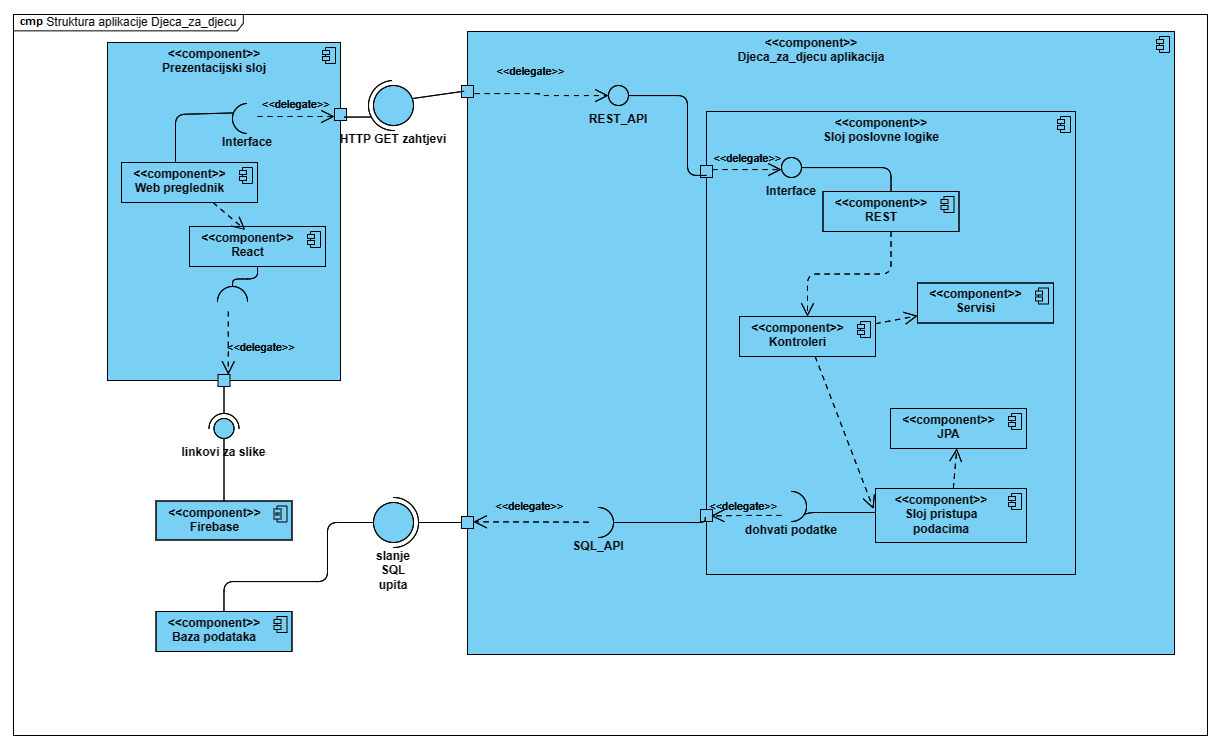
\includegraphics[width=\textwidth,height=0.5\textheight]{dijagrami/Dijagram_komponenti.png}%
				\centering
				\caption{Dijagram komponenti - struktura aplikacije}
				\label{fig:ComponentDiagram}
			\end{figure}		

		Na prezentacijskom sloju (frontendu) smještena je komponenta Web preglednik koja uz pomoć komponente React dohvaća i šalje stvari prema sustavu. Komponenta React koristi sučelje Firebase koje kreira linkove za slike koje možemo vidjeti u oglasima. Sustav također komunicira s Bazom podataka na kojoj su pohranjeni svi korisnički računi i oglasi. Na sloju poslovne logike nalaze se komponente koje vrše kompliciranije izračune, dohvat i izmjenu podataka iz baze i odgovaranje na zahtjeve pristigle s prezentacijskog sloja. Komunikacija izmedu prezentacijskog i sloja poslovne logike odvija se prema REST načelima. Za dohvaćanje podataka služi komponenta Sloj pristupa podacima preko koje se komunicira s Bazom podataka koja koristi JPA za prevodenje zahtjeva backenda u sintaksno ispravne SQL upite. Upiti se potom usmjeravaju prema bazi. Podaci zatim "putuju" natrag do frontenda i prikazujju se u pregledniku. 

			\eject

			%\textbf{\textit{dio 2. revizije}}\\
		
			% \textit{Potrebno je priložiti dijagram komponenti s pripadajućim opisom. Dijagram komponenti treba prikazivati strukturu cijele aplikacije.}